\documentclass[fleqn, a4paper. 12pt]{jsarticle} 
\usepackage{cite}
\usepackage{amsmath,txfonts}
\usepackage{amssymb}
\usepackage{url}
\usepackage[margin=31mm]{geometry}
\usepackage[dvipdfmx]{graphicx}
\usepackage{listings,jvlisting}
\usepackage{fancyhdr}
\usepackage{lastpage}
\usepackage{hyperref}
\usepackage[subrefformat=parens]{subcaption}
\lstset{
  basicstyle={\ttfamily},
  identifierstyle={\small},
  commentstyle={\smallitshape},
  keywordstyle={\small\bfseries},
  ndkeywordstyle={\small},
  stringstyle={\small\ttfamily},
  frame={tb},
  breaklines=true,
  columns=[l]{fullflexible},
  numbers=left,
  xrightmargin=0zw,
  xleftmargin=3zw,
  numberstyle={\scriptsize},
  stepnumber=1,
  numbersep=1zw,
  lineskip=-0.5ex
}
\renewcommand{\lstlistingname}{プログラム}

% header
\pagestyle{fancy}
\fancyhf{}
\rhead{2024-05}
\lhead{谷 知拓 - Tomohiro Tani}
\cfoot{\thepage\ / \pageref{LastPage}}

\geometry{left=25mm,right=25mm,top=25mm,bottom=30mm}

\begin{document}

  \begin{titlepage}
    \begin{center}
      {\Huge 2024年度\\応用プログラミング実験}
      
      \vspace{4cm}
      {\Huge 第9-11回\\デジタル信号処理\\
        実験レポート\\
      }
      \vspace{4cm}
      {\large 学修番号: 22140026\\谷 知拓 - Tomohiro Tani\footnote{東京都立大学 システムデザイン学部 情報科学科 \\ mail@taniii.com} \\}
      \vspace{0.5cm}
      {\large
        第1回レポート提出日 : 2024-06-12 \\
        第2回レポート提出日 : 2024-06-19 \\
        第3回レポート提出日 : 2024-06-27 \\
      }
    \end{center}
  \end{titlepage}

  \section*{はじめに}

    本レポートでは,『応用プログラミング実験』第9-11回デジタル信号処理の実施報告を行う.

  \subsection*{実験の概要}

    本実験では,デジタル信号処理について学ぶ.
    以下の課題に取り組み,その結果を報告する.

    \begin{enumerate}
      \item 課題1-1: 1Hz 正弦波
      \item 課題1-2: 周波数変化
      \item 課題1-3: 振幅変化
      \item 課題1-4: 周波数および位相変化
      \item 課題1-5: 直流変化
      \item 課題1-6: 信号の加算
      \item 課題1-7: 非周期信号
      \item 課題1-A: 追加課題
      \item 課題2-1: 和音の生成と再生
      \item 課題2-2: 和音のフーリエ解析
      \item 課題2-3: ディジタルフィルタの設計と適用
      \item 課題2-4: 様々なディジタルフィルタ
      \item 課題3-1: ナイキスト周波数
      \item 課題3-2: DFT と変換対
      \item 課題3-3: 窓関数
      \item 課題3-A: 応用問題
    \end{enumerate}

  \subsection*{実験環境}

    実験環境は以下の通りである.

    \begin{itemize}
      \item OS\footnote{Operating System}: macOS Ventura 13.4.1
      \item CPU\footnote{Central Processing Unit}: Apple M2 arm64\footnotemark[4]
      \item メインメモリ・ビデオメモリ共通: 16GBユニファイドメモリ\footnotemark[4]
      \footnotetext[4]{https://www.apple.com/jp/macbook-air-13-and-15-m2/specs/}
      \item 実行環境 (python3): Python 3.12.3
    \end{itemize}

  \newpage
  \section*{課題1-1: 1Hz 正弦波}

    条件は次の通りである.

    \begin{itemize}
      \item $T_0 = 1 [\mathrm{sec}]$
      \item $A = 1$
      \item $\theta = 0 [\mathrm{rad}]$
      \item $D = 0$
    \end{itemize}

    図 \ref{fig:s1} は,周期アナログ信号 $x_{T_0}(t)=A \sin \left(2 \pi F_0 t+\theta\right)+D$ および,その信号を標本化した離散時間信号 $x[n]$ をプロットしたものである.
    
    続いて,離散時間信号 $x[n]$ の離散フーリエスペクトル $X[k]$ を求めた.
    
    図 \ref{fign:a1} は,振幅スペクトル $|X[k]|$ を,図 \ref{fign:p1} は,位相スペクトル $\angle X[k][\mathrm{rad}]$ を示している.

    表 \ref{tab:1} は,周波数インデクス $k$ と各変数の対応表である.

    \begin{figure}[!h]
      \centering
      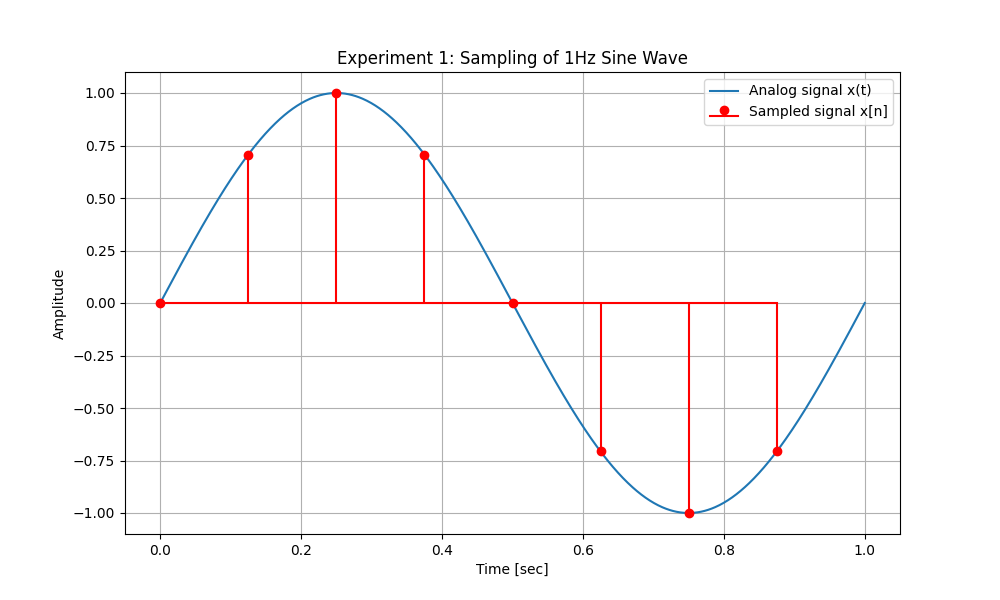
\includegraphics[width=0.6\textwidth]{sampling_experiment_1.png}
      \caption{周期アナログ信号 $x_{T_0}(t)$ とその信号を標本化した離散時間信号 $x[n]$}
      \label{fig:s1}
    \end{figure}

    \begin{figure}[h]
      \begin{center}
      \begin{minipage}[t]{0.48\columnwidth}
          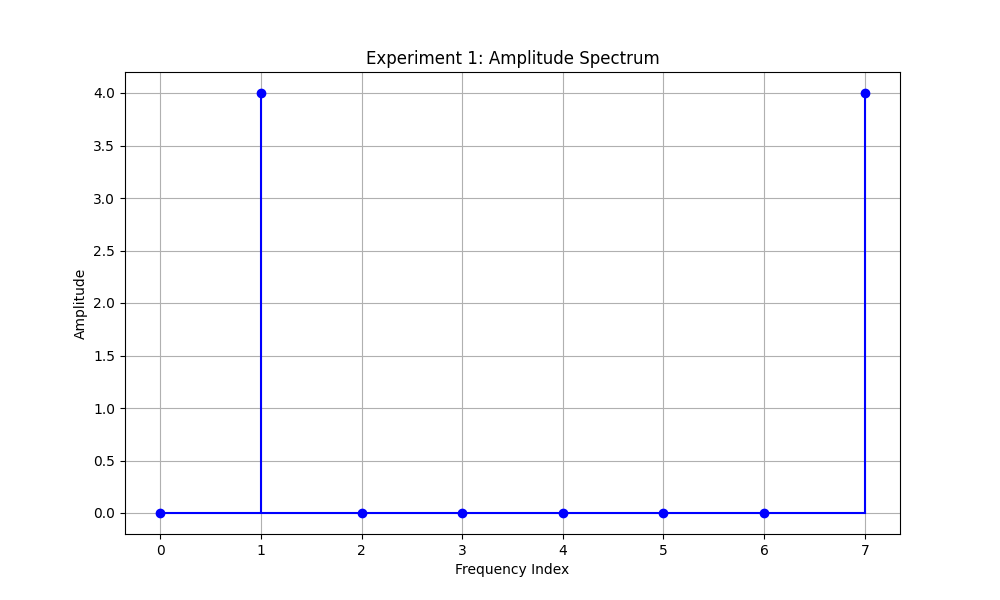
\includegraphics[width=\columnwidth]{amplitude_spectrum_experiment_1.png}
          \subcaption{振幅スペクトル $|X[k]|$}
          \label{fign:a1}
      \end{minipage}
      \begin{minipage}[t]{0.48\columnwidth}
          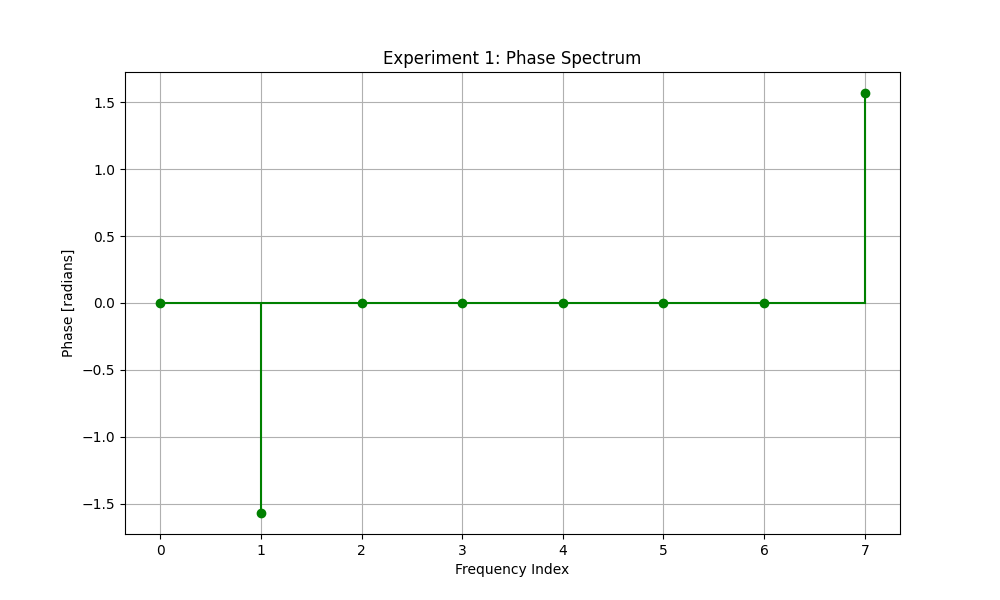
\includegraphics[width=\columnwidth]{phase_spectrum_experiment_1.png}
          \subcaption{位相スペクトル $\angle X[k][\mathrm{rad}]$}
          \label{fign:p1}
      \end{minipage}
      \end{center}
      \caption{離散時間信号 $x[n]$ の離散フーリエスペクトル $X[k]$}
    \end{figure}

    \begin{table}[!h]
      \centering
      \caption{周波数インデクス $k$ と各変数の対応表}
      \begin{tabular}{c|c|c|c|c|c|c|c|c}
        k & 0.0 & 1.0 & 2.0 & 3.0 & 4.0 & 5.0 & 6.0 & 7.0 \\
        \hline
        ω [rad] & 0.000000 & 0.785398 & 1.570796 & 2.356194 & 3.141593 & 3.926991 & 4.712389 & 5.497787 \\
        f & 0.000 & 0.125 & 0.250 & 0.375 & 0.500 & 0.625 & 0.750 & 0.875 \\
        Ω [rad/sec] & 0.000000 & 0.098175 & 0.196350 & 0.294524 & 0.392699 & 0.490874 & 0.589049 & 0.687223 \\
        F [Hz] & 0 & 1 & 2 & 3 & 4 & 5 & 6 & 7 
      \end{tabular}
      \label{tab:1}
    \end{table}

    \subsection*{考察}

      図 \ref{fign:a1} および,図 \ref{fign:p1} から,振幅スペクトル $|X[k]|$ は,周波数 $F$ が 1Hz のとき,$k=1, 7$ でピークを持ち,その他の周波数では 0 になっていることがわかる.

      また,位相スペクトル $\angle X[k][\mathrm{rad}]$ は,周波数 $F$ が 1Hz のとき,$k=1$ で位相が -1.5 rad を僅かに下回り, $k=7$ で位相が 1.5 rad を僅かに上回っていることが読み取れる.

      \quad

      離散フーリエ変換において,振幅スペクトルは,変換後の各周波数成分の大きさを表している.これは,信号のエネルギーがどの周波数にどのくらい含まれているかを示すものである.
      
      一方,位相スペクトルは,変換後の各周波数成分の位相を表している.これは,信号の各周波数成分がどの位相で現れているかを示すものである.

      これら,振幅スペクトルと位相スペクトルとを組み合わせることにより,元の信号を周波数領域で完全に表現することができ,時間領域と周波数領域の間の可逆変換を実現できる.

      \quad

      ここでは,$x_{T_0}(t)=A \sin \left(2 \pi F_0 t+\theta\right)+D$ をフーリエ変換している.
      
      連続な関数として,この変換を追うと次のようになる.

      時間領域信号:
      $$
      x_{T_0}(t) = A \sin \left(2 \pi F_0 t + \theta \right) + D
      $$

      この信号のフーリエ変換は次のように定義される:
      $$
      X(f) = \int_{-\infty}^{\infty} x_{T_0}(t) e^{-j 2 \pi f t} \, dt
      $$

      定数 \( D \) のフーリエ変換:
      $$
      \mathcal{F}\{ D \} = D \delta(f)
      $$

      正弦波 \( A \sin \left(2 \pi F_0 t + \theta \right) \) のフーリエ変換:
      $$
      \mathcal{F}\{ A \sin \left(2 \pi F_0 t + \theta \right) \} = \frac{A}{2j} \left[ e^{j \theta} \delta(f - F_0) - e^{-j \theta} \delta(f + F_0) \right]
      $$

      したがって、全体のフーリエ変換は次のようになる:
      $$
      X(f) = D \delta(f) + \frac{A}{2j} \left[ e^{j \theta} \delta(f - F_0) - e^{-j \theta} \delta(f + F_0) \right]
      $$

      この演繹により,振幅スペクトルおよび位相スペクトルのピークの理論値は以下のようにいえる.

      \subsection*{振幅スペクトルのピーク}
        \begin{itemize}
            \item \( f = 0 \) において \( |X(0)| = |D| \)
            \item \( f = \pm F_0 \) において \( |X(\pm F_0)| = \frac{A}{2} \)
        \end{itemize}

        \subsection*{位相スペクトルのピーク}
        \begin{itemize}
            \item \( f = 0 \) において位相は \( 0 \)
            \item \( f = F_0 \) において位相は \( \theta + \frac{\pi}{2} \)
            \item \( f = -F_0 \) において位相は \( -\theta - \frac{\pi}{2} \)
      \end{itemize}

      ここで,離散フーリエ変換を行った今回の実験と比較する.

      まず,連続な関数におけるフーリエ変換と離散な関数におけるフーリエ変換の違いについて考える.

      連続な関数のフーリエ変換では,$0$ を中心として対象にスペクトルが 1 周期分のみ現れる.

      一方,離散な関数のフーリエ変換では,サンプリング数を周期とする,周期的なスペクトルが現れる.

      そこで,今回の実験結果に注目すると,スペクトルは $k = 1, 7$ にピークが現れている.
      
      このスペクトルは周期的であることから,$k = 7$ のピークは,1 つ前の周期では,$k = -1$ にピークが現れている.

      このことから,振幅スペクトルおよび位相スペクトルのピークは,理論値と一致していることがわかる.

      \quad

      次に,振幅スペクトルおよび位相スペクトルのピークにおける値を考える.

      振幅スペクトルのピークにおける値は,$A$ とサンプリング数に依存する.

      今回の実験では,$A = 1$ であるため,振幅スペクトルのピークにおける値は $\frac{A}{2} \times 8$ を計算することにより,$4$ となり,これは実験結果と一致する.

      また,位相スペクトルのピークにおける値は,$\theta$ に依存する.

      今回の実験では,$\theta = 0$ であるため,位相スペクトルのピークにおける値は $\theta \pm \frac{\pi}{2} = \pm \frac{\pi}{2}$ となり,これは実験結果と一致する.

      よって,今回の実験結果を通して,フーリエ変換における振幅スペクトルおよび位相スペクトルが連続関数における理論値と一致していることが確認できた.
  
  \newpage
  \section*{課題1-2: 周波数変化}

  条件は次の通りである.

  \begin{itemize}
    \item $T_0 = 1/2 [\mathrm{sec}]$
    \item $A = 1$
    \item $\theta = 0 [\mathrm{rad}]$
    \item $D = 0$
  \end{itemize}

  図 \ref{fig:s2} は,周期アナログ信号 $x_{T_0}(t)=A \sin \left(2 \pi F_0 t+\theta\right)+D$ および,その信号を標本化した離散時間信号 $x[n]$ をプロットしたものである.

  続いて,離散時間信号 $x[n]$ の離散フーリエスペクトル $X[k]$ を求めた.

  図 \ref{fign:a2} は,振幅スペクトル $|X[k]|$ を,図 \ref{fign:p2} は,位相スペクトル $\angle X[k][\mathrm{rad}]$ を示している.

  \begin{figure}[!h]
    \centering
    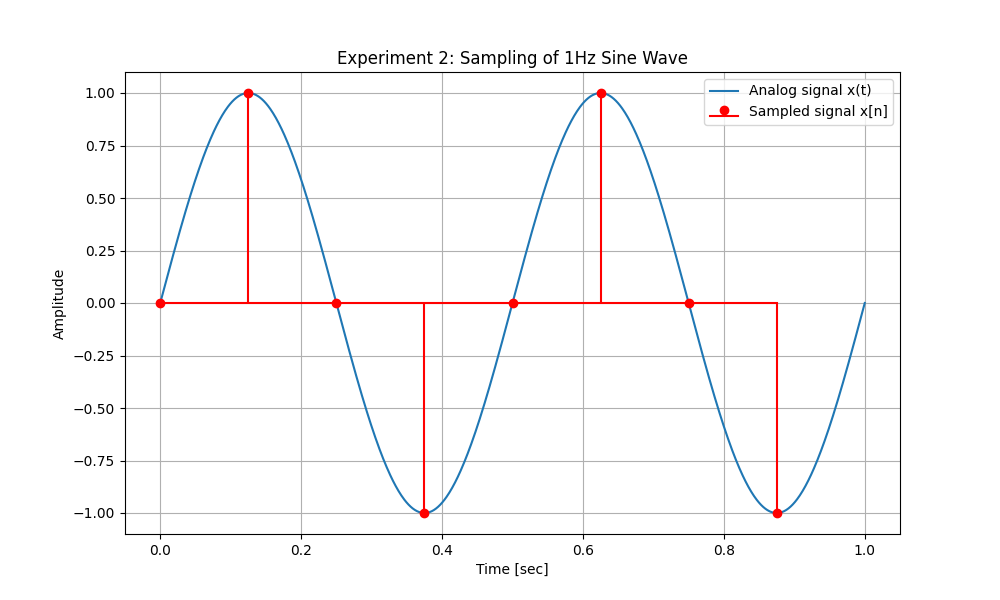
\includegraphics[width=0.6\textwidth]{sampling_experiment_2.png}
    \caption{周期アナログ信号 $x_{T_0}(t)$ とその信号を標本化した離散時間信号 $x[n]$}
    \label{fig:s2}
  \end{figure}

  \begin{figure}[h]
    \begin{center}
    \begin{minipage}[t]{0.48\columnwidth}
        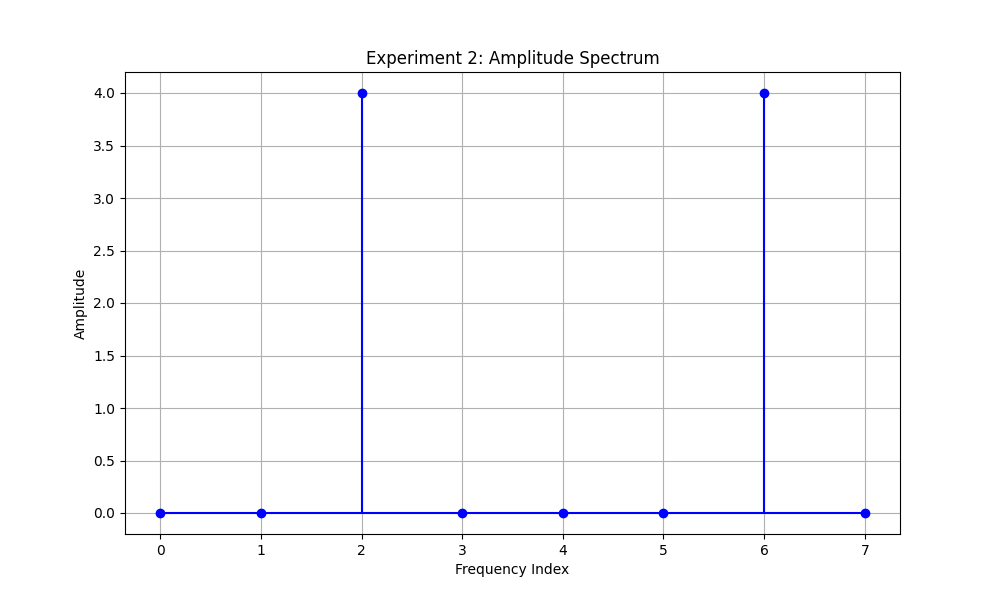
\includegraphics[width=\columnwidth]{amplitude_spectrum_experiment_2.png}
        \subcaption{振幅スペクトル $|X[k]|$}
        \label{fign:a2}
    \end{minipage}
    \begin{minipage}[t]{0.48\columnwidth}
        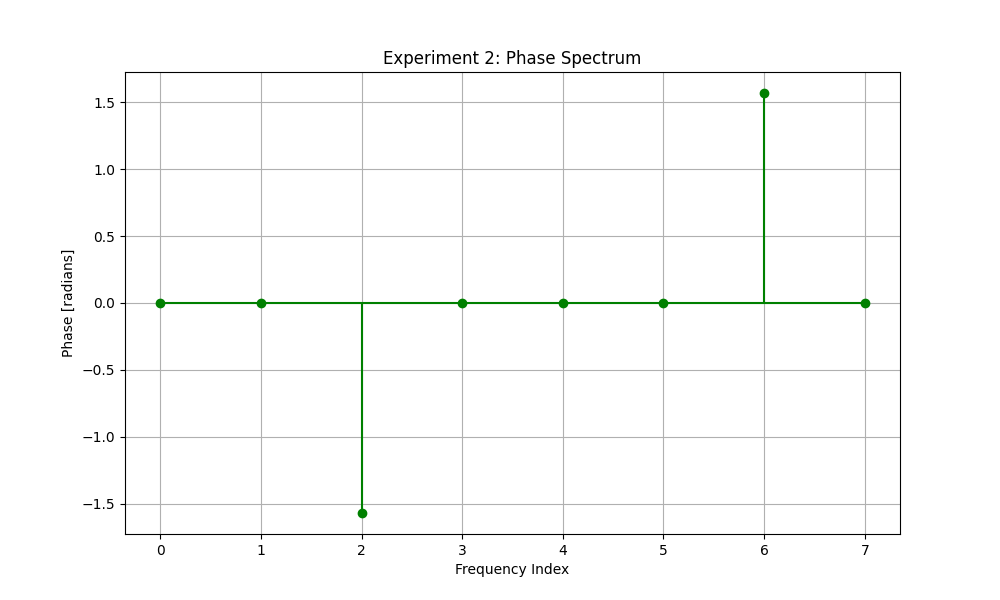
\includegraphics[width=\columnwidth]{phase_spectrum_experiment_2.png}
        \subcaption{位相スペクトル $\angle X[k][\mathrm{rad}]$}
        \label{fign:p2}
    \end{minipage}
    \end{center}
    \caption{離散時間信号 $x[n]$ の離散フーリエスペクトル $X[k]$}
  \end{figure}

  \subsection*{考察}

    課題 1-1 と比較すると,$T_0 = 1$ から $T_0 = 1/2$ に変化したことで,周波数 $F$ が 1Hz から 2Hz に変化している.

    これにより,振幅スペクトル $|X[k]|$ は,周波数 $F$ が 2Hz のとき,$k=2, 6$ でピークを持ち,その他の周波数では 0 になっていることがわかる.

    また,位相スペクトル $\angle X[k][\mathrm{rad}]$ は,周波数 $F$ が 2Hz のとき,$k=2$ で位相が -1.5 rad を僅かに下回り, $k=6$ で位相が 1.5 rad を僅かに上回っていることが読み取れる.

    これらのことから,元の信号の周波数が変化したことにより,スペクトルのピークが生じる周波数も変化したといえる.

  \newpage

  \section*{課題1-3: 振幅変化}
    
  条件は次の通りである.

  \begin{itemize}
    \item $T_0 = 1 [\mathrm{sec}]$
    \item $A = 2$
    \item $\theta = 0 [\mathrm{rad}]$
    \item $D = 0$
  \end{itemize}

  図 \ref{fig:s3} は,周期アナログ信号 $x_{T_0}(t)=A \sin \left(2 \pi F_0 t+\theta\right)+D$ および,その信号を標本化した離散時間信号 $x[n]$ をプロットしたものである.

  続いて,離散時間信号 $x[n]$ の離散フーリエスペクトル $X[k]$ を求めた.

  図 \ref{fign:a3} は,振幅スペクトル $|X[k]|$ を,図 \ref{fign:p3} は,位相スペクトル $\angle X[k][\mathrm{rad}]$ を示している.

  \begin{figure}[!h]
    \centering
    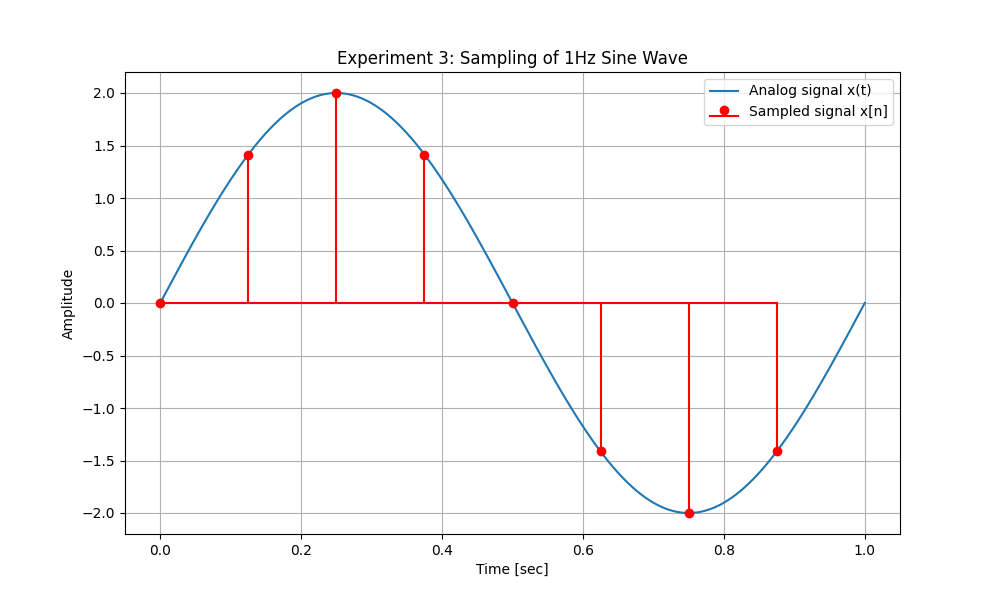
\includegraphics[width=0.6\textwidth]{sampling_experiment_3.png}
    \caption{周期アナログ信号 $x_{T_0}(t)$ とその信号を標本化した離散時間信号 $x[n]$}
    \label{fig:s3}
  \end{figure}

  \begin{figure}[h]
    \begin{center}
    \begin{minipage}[t]{0.48\columnwidth}
        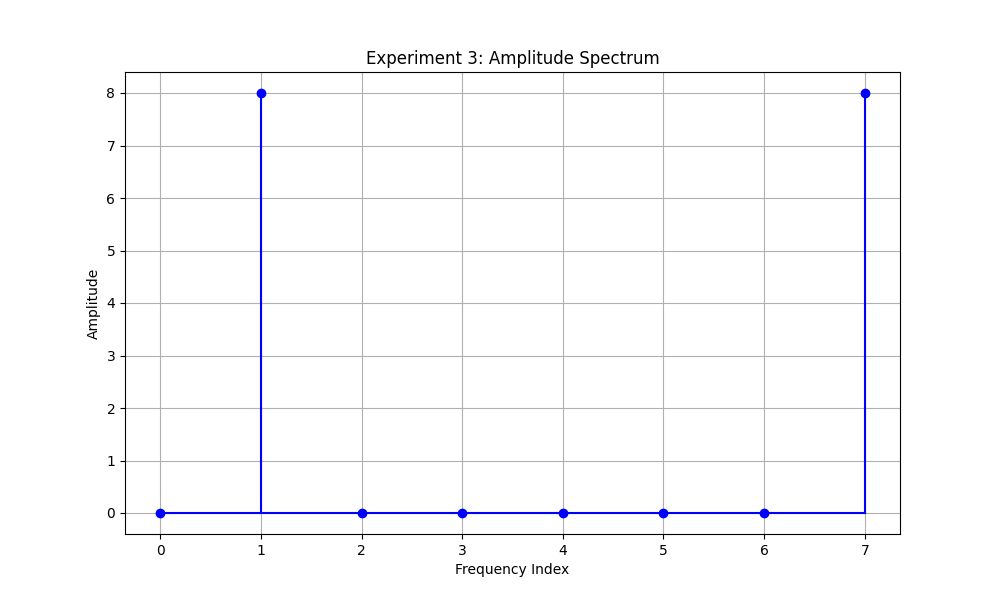
\includegraphics[width=\columnwidth]{amplitude_spectrum_experiment_3.png}
        \subcaption{振幅スペクトル $|X[k]|$}
        \label{fign:a3}
    \end{minipage}
    \begin{minipage}[t]{0.48\columnwidth}
        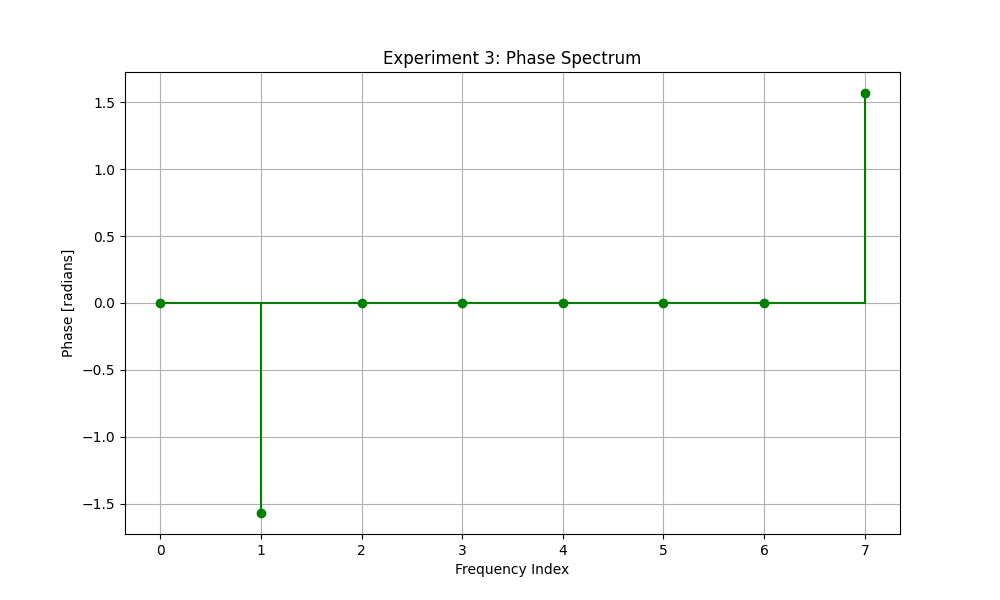
\includegraphics[width=\columnwidth]{phase_spectrum_experiment_3.png}
        \subcaption{位相スペクトル $\angle X[k][\mathrm{rad}]$}
        \label{fign:p3}
    \end{minipage}
    \end{center}
    \caption{離散時間信号 $x[n]$ の離散フーリエスペクトル $X[k]$}
  \end{figure}

  \subsection*{考察}

    課題 1-1, 1-2 と比較すると,$A = 1$ から $A = 2$ に変化したことで,振幅が 1 から 2 に変化している.

    これにより,振幅スペクトル $|X[k]|$ は,周波数 $F$ が 1Hz のとき,$k=1, 7$ でピークを持ち,その振幅はそれぞれ 8 となっている.

    これらのことから,元の信号の振幅が変化したことにより,スペクトルのピークの振幅も変化したといえる.

  \newpage

  \section*{課題1-4: 周波数および位相変化}

  条件は次の通りである.

  \begin{itemize}
    \item $T_0 = 1/2 [\mathrm{sec}]$
    \item $A = 1$
    \item $\theta = \pi [\mathrm{rad}]$
    \item $D = 0$
  \end{itemize}

  図 \ref{fig:s4} は,周期アナログ信号 $x_{T_0}(t)=A \sin \left(2 \pi F_0 t+\theta\right)+D$ および,その信号を標本化した離散時間信号 $x[n]$ をプロットしたものである.

  続いて,離散時間信号 $x[n]$ の離散フーリエスペクトル $X[k]$ を求めた.

  図 \ref{fign:a4} は,振幅スペクトル $|X[k]|$ を,図 \ref{fign:p4} は,位相スペクトル $\angle X[k][\mathrm{rad}]$ を示している.

  \begin{figure}[!h]
    \centering
    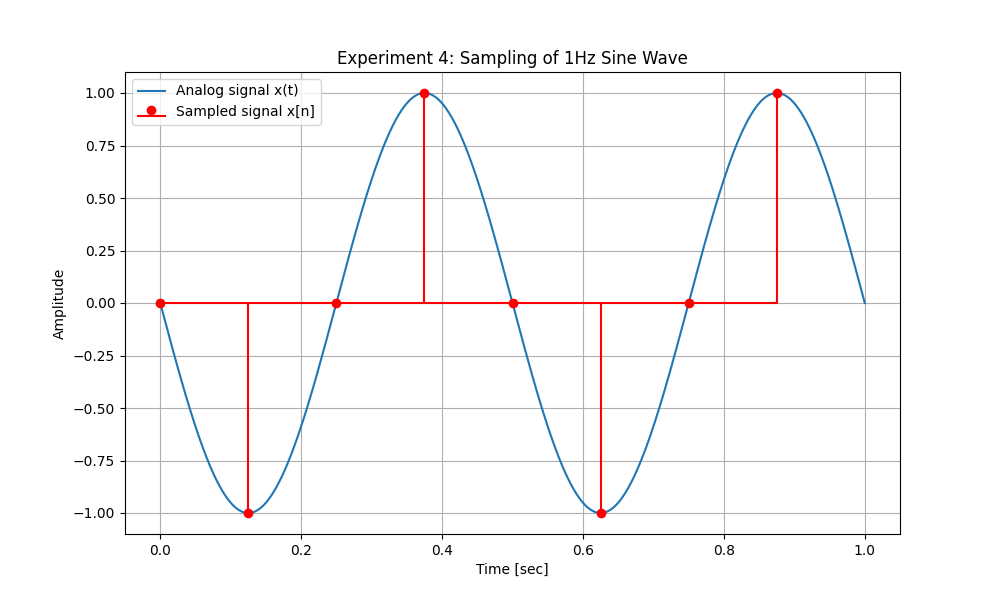
\includegraphics[width=0.6\textwidth]{sampling_experiment_4.png}
    \caption{周期アナログ信号 $x_{T_0}(t)$ とその信号を標本化した離散時間信号 $x[n]$}
    \label{fig:s4}
  \end{figure}

  \begin{figure}[h]
    \begin{center}
    \begin{minipage}[t]{0.48\columnwidth}
        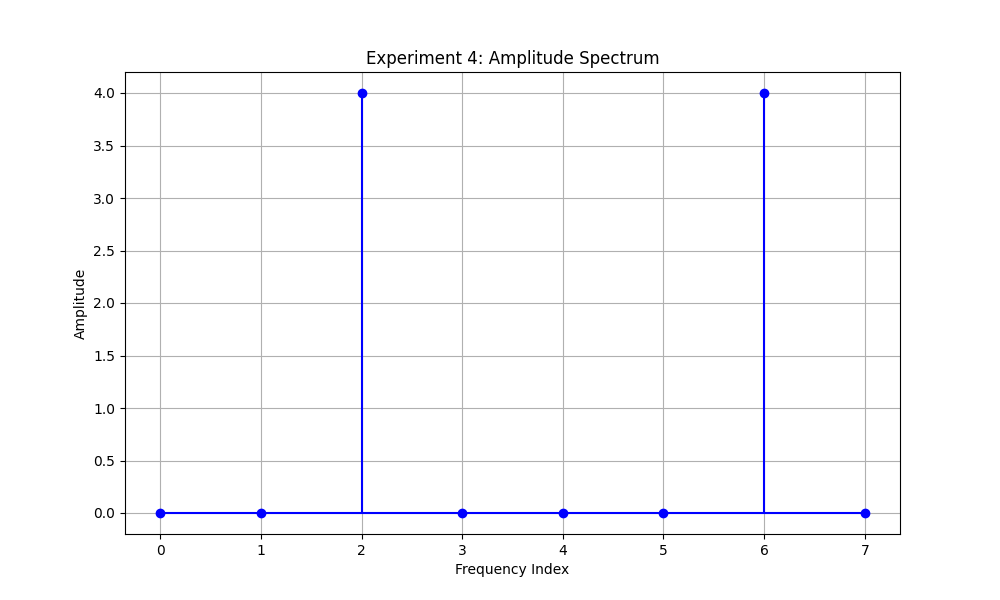
\includegraphics[width=\columnwidth]{amplitude_spectrum_experiment_4.png}
        \subcaption{振幅スペクトル $|X[k]|$}
        \label{fign:a4}
    \end{minipage}
    \begin{minipage}[t]{0.48\columnwidth}
        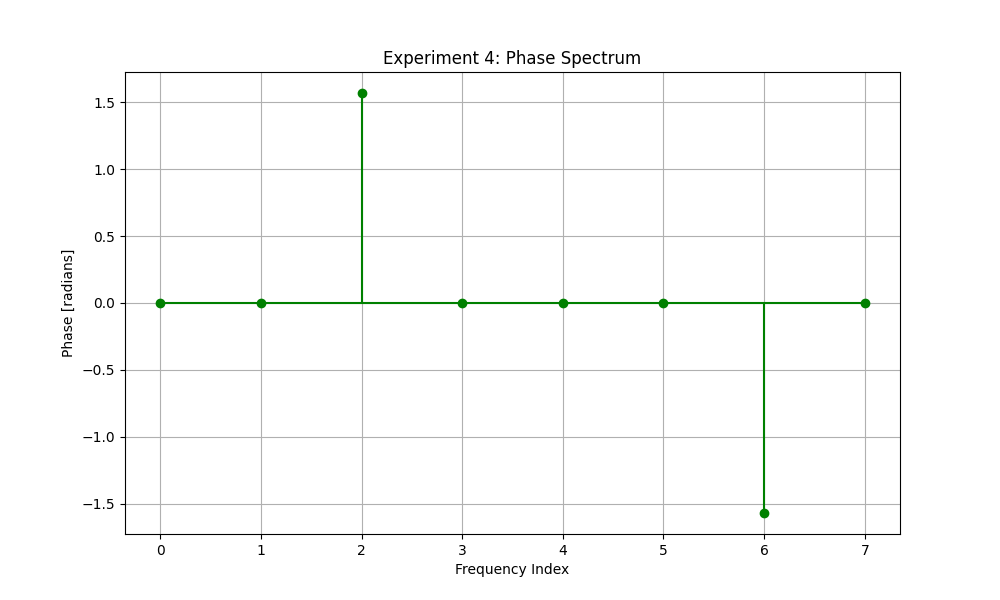
\includegraphics[width=\columnwidth]{phase_spectrum_experiment_4.png}
        \subcaption{位相スペクトル $\angle X[k][\mathrm{rad}]$}
        \label{fign:p4}
    \end{minipage}
    \end{center}
    \caption{離散時間信号 $x[n]$ の離散フーリエスペクトル $X[k]$}
  \end{figure}

  \subsection*{考察}

    課題 1-1, 1-2, 1-3 と比較すると,$\theta = 0$ から $\theta = \pi$ に変化したことで,位相が 0 から $\pi$ に変化している.

    これにより,位相スペクトル $\angle X[k][\mathrm{rad}]$ は,周波数 $F$ が 2Hz のとき,$k=2$ で位相が 1.5 rad を僅かに上回っており, $k=6$ で位相が -1.5 rad を僅かに下回っていることが読み取れる.

    これらのことから,元の信号の位相が変化したことにより,スペクトルのピークの位相も変化したといえる.

  \newpage

  \section*{課題1-5: 直流変化}

  条件は次の通りである.

  \begin{itemize}
    \item $T_0 = 1 [\mathrm{sec}]$
    \item $A = 1$
    \item $\theta = 0 [\mathrm{rad}]$
    \item $D = 1$
  \end{itemize}

  図 \ref{fig:s5} は,周期アナログ信号 $x_{T_0}(t)=A \sin \left(2 \pi F_0 t+\theta\right)+D$ および,その信号を標本化した離散時間信号 $x[n]$ をプロットしたものである.

  続いて,離散時間信号 $x[n]$ の離散フーリエスペクトル $X[k]$ を求めた.

  図 \ref{fign:a5} は,振幅スペクトル $|X[k]|$ を,図 \ref{fign:p5} は,位相スペクトル $\angle X[k][\mathrm{rad}]$ を示している.

  \begin{figure}[!h]
    \centering
    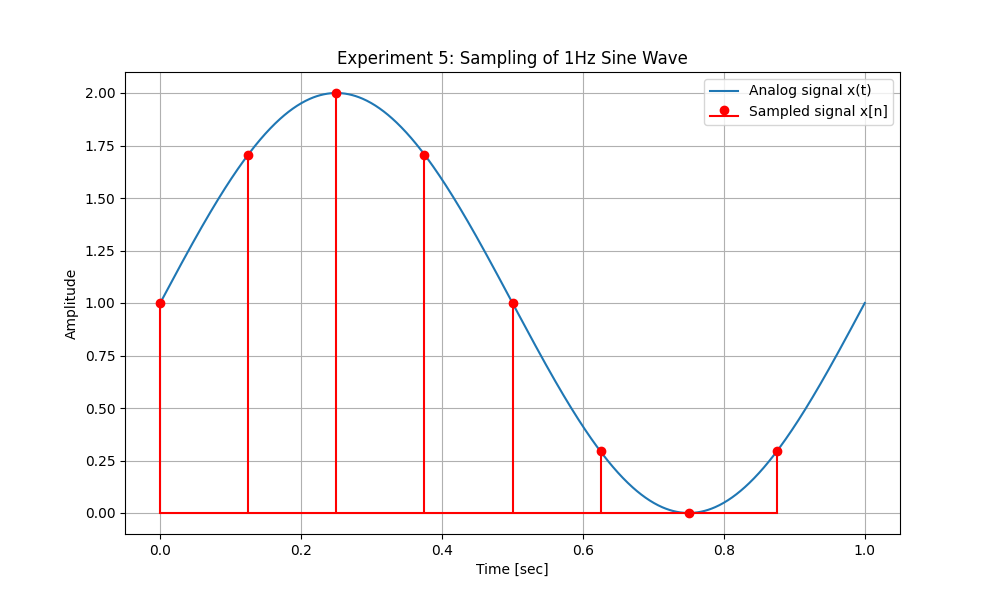
\includegraphics[width=0.6\textwidth]{sampling_experiment_5.png}
    \caption{周期アナログ信号 $x_{T_0}(t)$ とその信号を標本化した離散時間信号 $x[n]$}
    \label{fig:s5}
  \end{figure}

  \begin{figure}[h]
    \begin{center}
    \begin{minipage}[t]{0.48\columnwidth}
        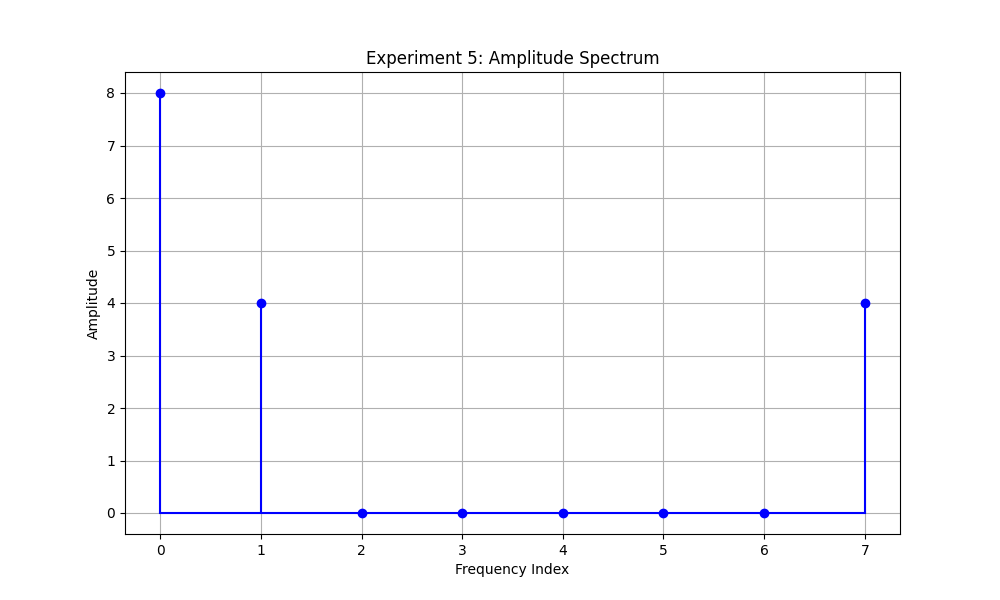
\includegraphics[width=\columnwidth]{amplitude_spectrum_experiment_5.png}
        \subcaption{振幅スペクトル $|X[k]|$}
        \label{fign:a5}
    \end{minipage}
    \begin{minipage}[t]{0.48\columnwidth}
        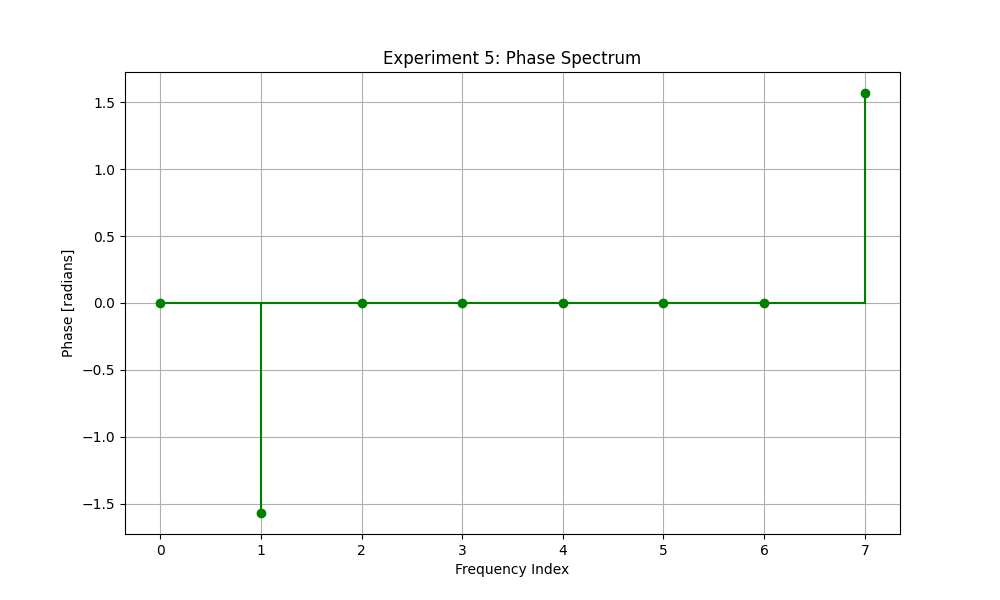
\includegraphics[width=\columnwidth]{phase_spectrum_experiment_5.png}
        \subcaption{位相スペクトル $\angle X[k][\mathrm{rad}]$}
        \label{fign:p5}
    \end{minipage}
    \end{center}
    \caption{離散時間信号 $x[n]$ の離散フーリエスペクトル $X[k]$}
  \end{figure}

  \subsection*{考察}

    課題 1-1 と比較すると,$D = 0$ から $D = 1$ に変化したことで,直流成分が 0 から 1 に変化している.

    これにより,振幅スペクトル $|X[k]|$ は,周波数 $F$ が 1Hz のとき,$k=0, 1, 7$ でピークを持ち,その振幅はそれぞれ 8, 4, 4 となっている.

    これらのことから,元の信号の直流成分が変化したことにより,スペクトルのピークの振幅も変化したといえる.

  \newpage

  \section*{課題1-6: 信号の加算}

  条件は次の通りである.

  \begin{itemize}
    \item $T_0 = 1 [\mathrm{sec}]$
  \end{itemize}

  図 \ref{fig:s6} は,周期アナログ信号 $a_{T_0}(t)=2 \sin (2 \pi t)+\sin (4 \pi t+\pi)$ および,その信号を標本化した離散時間信号 $a[n]$ をプロットしたものである.

  続いて,離散時間信号 $a[n]$ の離散フーリエスペクトル $X[k]$ を求めた.

  図 \ref{fign:a6} は,振幅スペクトル $|X[k]|$ を,図 \ref{fign:p6} は,位相スペクトル $\angle X[k][\mathrm{rad}]$ を示している.

  \begin{figure}[!h]
    \centering
    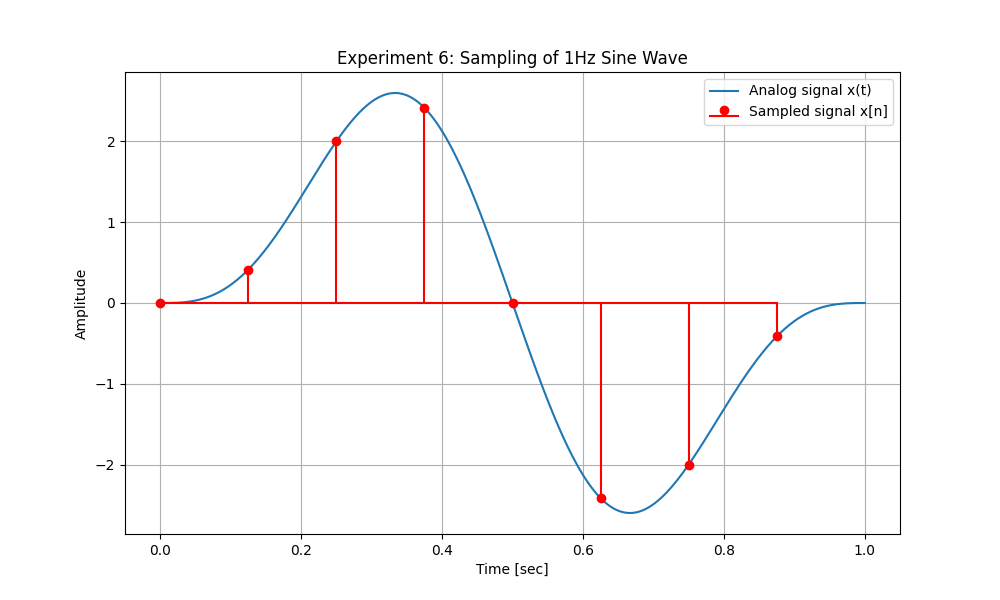
\includegraphics[width=0.6\textwidth]{sampling_experiment_6.png}
    \caption{周期アナログ信号 $x_{T_0}(t)$ とその信号を標本化した離散時間信号 $x[n]$}
    \label{fig:s6}
  \end{figure}

  \begin{figure}[h]
    \begin{center}
    \begin{minipage}[t]{0.48\columnwidth}
        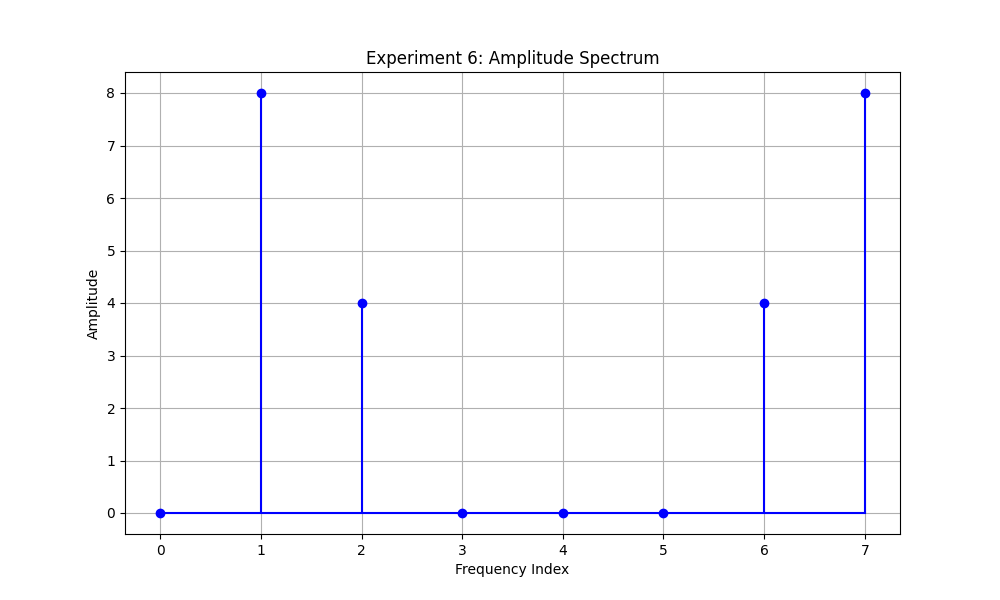
\includegraphics[width=\columnwidth]{amplitude_spectrum_experiment_6.png}
        \subcaption{振幅スペクトル $|X[k]|$}
        \label{fign:a6}
    \end{minipage}
    \begin{minipage}[t]{0.48\columnwidth}
        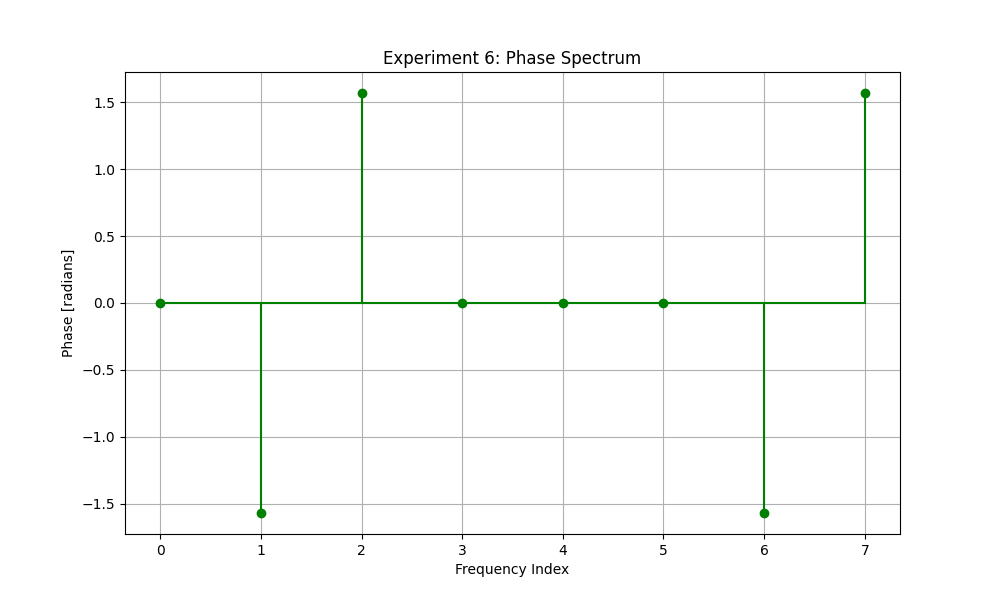
\includegraphics[width=\columnwidth]{phase_spectrum_experiment_6.png}
        \subcaption{位相スペクトル $\angle X[k][\mathrm{rad}]$}
        \label{fign:p6}
    \end{minipage}
    \end{center}
    \caption{離散時間信号 $x[n]$ の離散フーリエスペクトル $X[k]$}
  \end{figure}

  \subsection*{考察}

    課題 1-2, 1-3, 1-4 と比較すると,この事件では,$a_{T_0}(t)=2 \sin (2 \pi t)+\sin (4 \pi t+\pi)$ というように 2 つの波の合成波になっており,周波数 $F$ が 2Hz および 4Hz の信号が混在している.

    よって,スペクトルのピークは,$k = 1, 2, 6, 7$ に生じており,それぞれのピークの振幅は 8, 4, 4, 8 となっている.

    2 つの周波数の波からなる合成波のため,スペクトルのピークが 4 箇所に生じていることがわかる.

  \newpage

  \section*{課題1-7: 非周期信号}

  条件は次の通りである.

  \begin{itemize}
    \item $T_0 = 0.8 [\mathrm{sec}]$
    \item $A = 1$
    \item $\theta = 1 [\mathrm{rad}]$
    \item $D = 0$
  \end{itemize}

  図 \ref{fig:s7} は,周期アナログ信号 $x_{T_0}(t)=A \sin \left(2 \pi F_0 t+\theta\right)+D$ および,その信号を標本化した離散時間信号 $x[n]$ をプロットしたものである.
  
  続いて,離散時間信号 $x[n]$ の離散フーリエスペクトル $X[k]$ を求めた.
  
  図 \ref{fign:a7} は,振幅スペクトル $|X[k]|$ を,図 \ref{fign:p7} は,位相スペクトル $\angle X[k][\mathrm{rad}]$ を示している.

  \begin{figure}[!h]
    \centering
    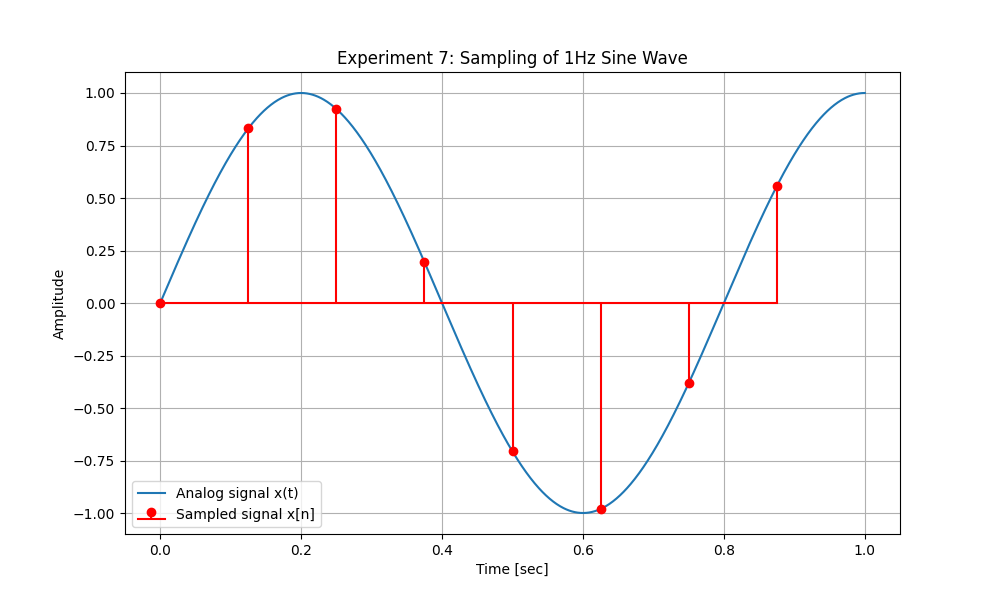
\includegraphics[width=0.6\textwidth]{sampling_experiment_7.png}
    \caption{周期アナログ信号 $x_{T_0}(t)$ とその信号を標本化した離散時間信号 $x[n]$}
    \label{fig:s7}
  \end{figure}

  \begin{figure}[h]
    \begin{center}
    \begin{minipage}[t]{0.48\columnwidth}
        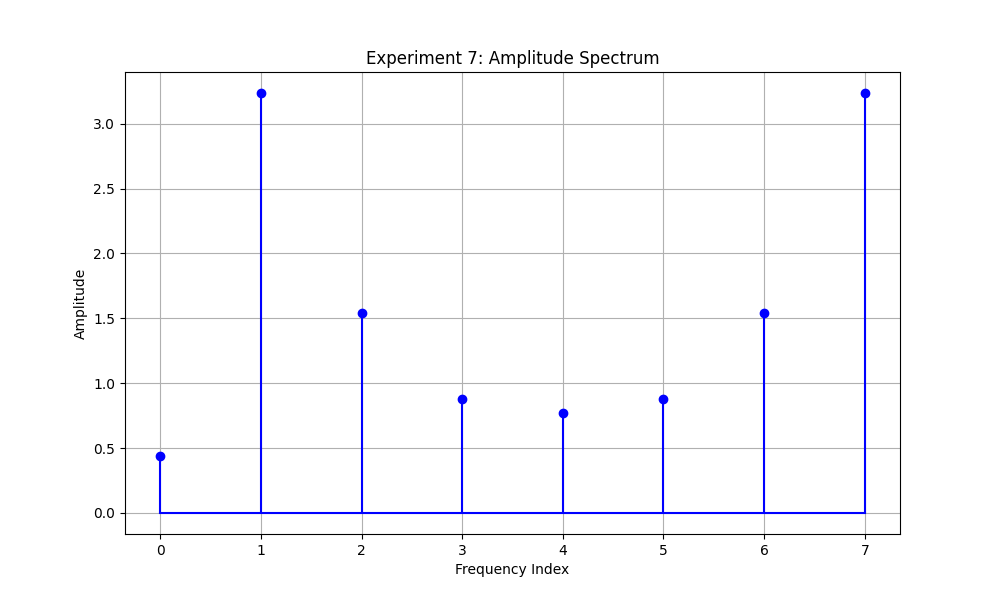
\includegraphics[width=\columnwidth]{amplitude_spectrum_experiment_7.png}
        \subcaption{振幅スペクトル $|X[k]|$}
        \label{fign:a7}
    \end{minipage}
    \begin{minipage}[t]{0.48\columnwidth}
        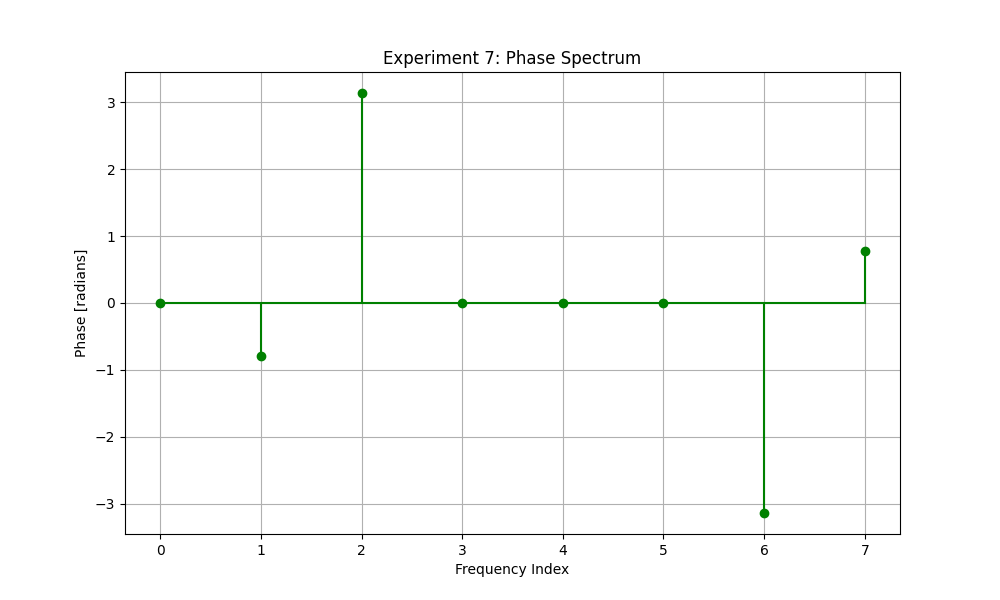
\includegraphics[width=\columnwidth]{phase_spectrum_experiment_7.png}
        \subcaption{位相スペクトル $\angle X[k][\mathrm{rad}]$}
        \label{fign:p7}
    \end{minipage}
    \end{center}
    \caption{離散時間信号 $x[n]$ の離散フーリエスペクトル $X[k]$}
  \end{figure}

  \subsection*{考察}

    課題 1-1 と比較すると,非周期信号のため,周期性がない.

    そのため,スペクトルのピークは,$k = 1, 2, 3, 4, 5, 6, 7$ に生じている.

    これは,非周期信号のため,周波数が連続的に変化しているためであるといえる.

  \newpage
  \section*{課題2-1: 和音の生成と再生}

  条件は次の通りである.

  \begin{itemize}
    \item ラ ($ = 440 [\mathrm{Hz}]$) および ド ($ = 261.626 [\mathrm{Hz}]$) の音を合成した音を生成する.
  \end{itemize}

  図 \ref{fig:fig1} は,生成した離散時間信号 $x_1[n]$, $x_2[n]$, $x_add[n]$ をプロットしたものである.

  \begin{figure}[!h]
    \centering
    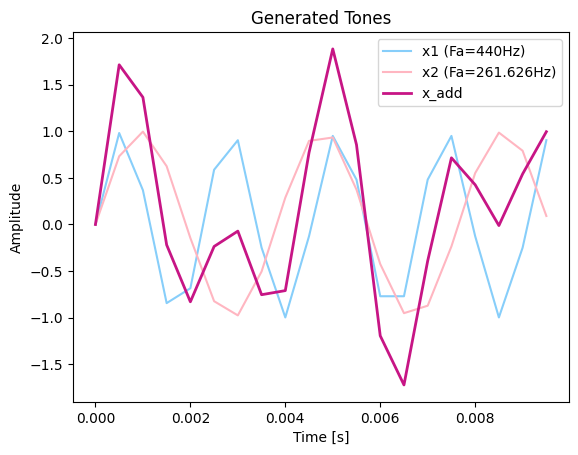
\includegraphics[width=0.6\textwidth]{fig_1.png}
    \caption{生成した離散時間信号 $x_1[n]$, $x_2[n]$, $x_add[n]$}
    \label{fig:fig1}
  \end{figure}

  \newpage
  \section*{課題2-2: 和音のフーリエ解析}

  図 \ref{fig:fig3} , 図 \ref{fig:fig4}, 図 \ref{fig:fig2} は, $x_1[n]$, $x_2[n]$, $x_add[n]$ それぞれに $N = 2000$ 点の離散時間フーリエ変換をかけ,得られた振幅スペクトルをプロットしたものである.

  \begin{figure}[h]
    \begin{center}
    \begin{minipage}[t]{0.48\columnwidth}
        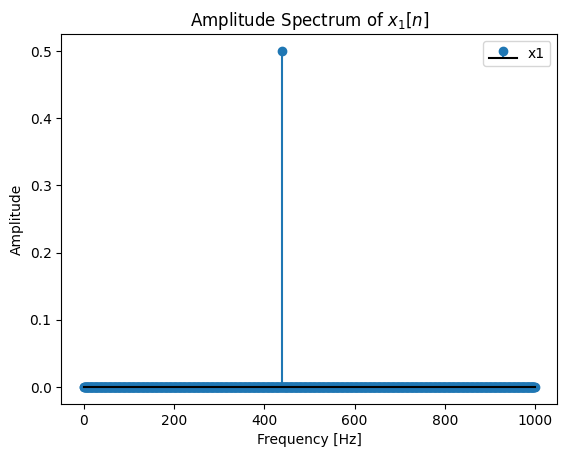
\includegraphics[width=\columnwidth]{fig_23.png}
        \subcaption{振幅スペクトル $|X_1[k]|$}
        \label{fig:fig3}
    \end{minipage}
    \begin{minipage}[t]{0.48\columnwidth}
      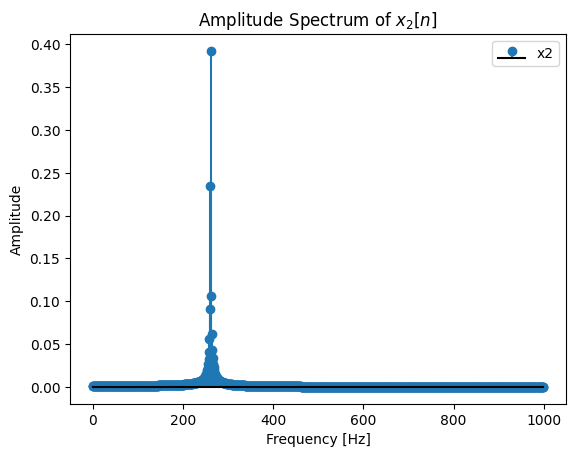
\includegraphics[width=\columnwidth]{fig_24.png}
      \subcaption{振幅スペクトル $|X_2[k]|$}
      \label{fig:fig4}
    \end{minipage}
    \begin{minipage}[t]{0.48\columnwidth}
      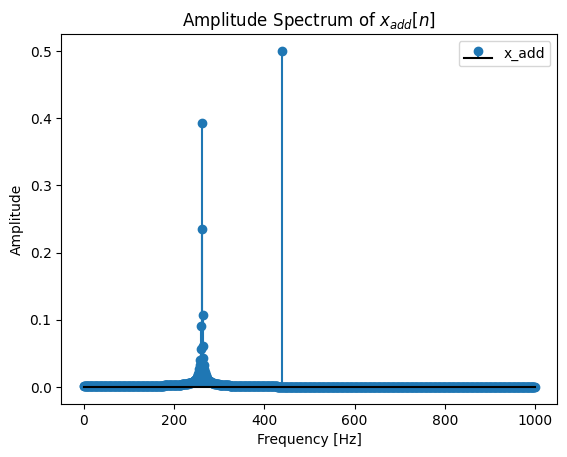
\includegraphics[width=\columnwidth]{fig_22.png}
      \subcaption{振幅スペクトル $|X_add[k]|$}
      \label{fig:fig2}
    \end{minipage}
    \end{center}
    \caption{$x_1[n]$, $x_2[n]$, $x_add[n]$ それぞれに $N = 2000$ 点の離散時間フーリエ変換をかけ,得られた振幅スペクトル}
  \end{figure}

  \subsection*{考察}

    和音は,ラ ($ = 440 [\mathrm{Hz}]$) および ド ($ = 261.626 [\mathrm{Hz}]$) の音を合成したものである.

    加算信号の離散時間フーリエ変換の振幅スペクトル $|X_{\text{add}}[k]|$ は,周波数 $F$ が 440Hz および 261.626Hz のときピークを持っており,これは,$x_1[n]$ および $x_2[n]$ の振幅スペクトル $|X_1[k]|$, $|X_2[k]|$ と一致している.

    このことから,和音が複数の音を合成したものであるため,それぞれの周波数成分が加算されていることがわかる.

  \newpage
  \section*{課題2-3: ディジタルフィルタの設計と適用}

  図 \ref{fig:fig5} は, 作成したローパスフィルタ $h_lpf[n]$ を $N = 2000$ 点の離散時間フーリエ変換をかけ,得られた振幅スペクトル $|h=H_lpf[k]|$ をプロットしたものである.

  ただし,ローパスフィルタ $h_lpf[n]$ は,通過域端周波数 $F_{pass} = 360 [\mathrm{Hz}]$,阻止域端周波数 $F_{stop} = 440 [\mathrm{Hz}]$ とした.

  \begin{figure}[!h]
    \centering
    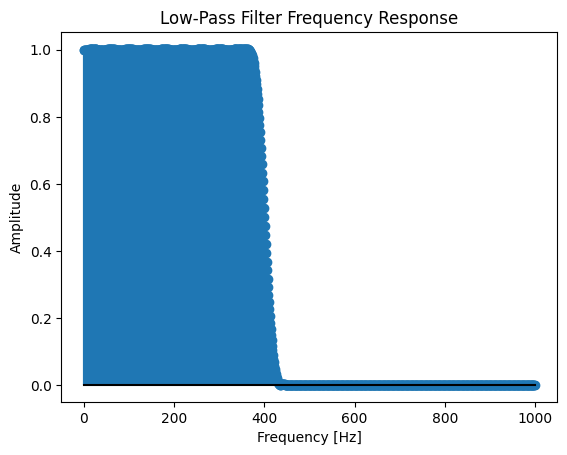
\includegraphics[width=0.6\textwidth]{fig_25.png}
    \caption{作成したローパスフィルタ $h_lpf[n]$ の振幅スペクトル $H_lpf[k]$}
    \label{fig:fig5}
  \end{figure}

  次に,図 \ref{fig:fig6} は, $x_{add}[n]$ に,作成したローパスフィルタ $h_lpf[n]$ を適用し得た,畳み込み和 $y[n]$ について,$N = 2000$ 点のフーリエ変換をかけ,得られた振幅スペクトル $|Y[n]|$ をプロットしたものである.

  \begin{figure}[!h]
    \centering
    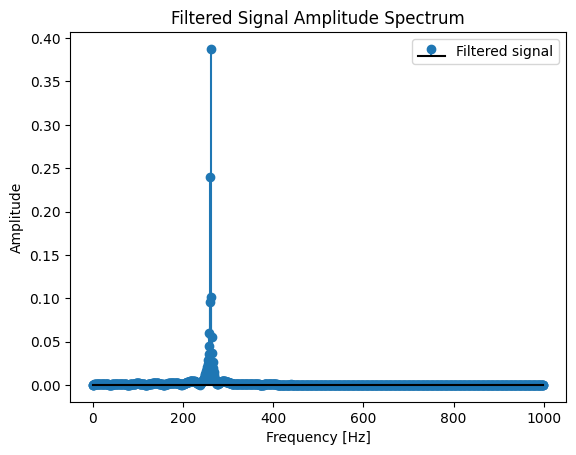
\includegraphics[width=0.6\textwidth]{fig_26.png}
    \caption{畳み込み和 $y[n]$ の振幅スペクトル $|Y[n]|$}
    \label{fig:fig6}
  \end{figure}

  \subsection*{考察}

    作成したローパスフィルタ $h_lpf[n]$ は,通過域端周波数 $F_{pass} = 360 [\mathrm{Hz}]$,阻止域端周波数 $F_{stop} = 440 [\mathrm{Hz}]$ とした.

    図 \ref{fig:fig5} より,$F = 360 [\mathrm{Hz}]$ 以下の周波数成分は確実に通過し,$F = 440[\mathrm{Hz}]$ 以上の周波数成分が確実にカットされることがわかる.

    図 \ref{fig:fig6} を,課題2-2 の $|X_{add}[n]|$ の図 \ref{fig:fig2} と比較すると, $F = 360 [\mathrm{Hz}]$ 以下のド ($ = 261.626 [\mathrm{Hz}]$) に対応する位相スペクトルのピークは残され,ラ ($ = 440 [\mathrm{Hz}]$) に対応する位相スペクトルのピークはカットされていることが確認できる.

    このことから,ローパスフィルタが正しく設計され,適用されていることがわかる.

  \newpage
  
  \section*{課題2-4: 様々なディジタルフィルタ}

    ハイパスフィルタ $h_hpf[n]$ および,バンドパスフィルタ $h_bpf[n]$ を設計した.

    ただし,ハイパスフィルタは,通過域端周波数 $F_{pass} = 440 [\mathrm{Hz}]$,阻止域端周波数 $F_{pass} = 360 [\mathrm{Hz}]$ とし,バンドパスフィルタは,周波数の低い方から,阻止域端周波数 $F_{lstop} = 160 [\mathrm{Hz}]$,通過域端周波数 $F_{lpass} = 260 [\mathrm{Hz}]$ ,通過域端周波数 $F_{hpass} = 540 [\mathrm{Hz}]$,阻止域端周波数 $F_{hstop} = 640 [\mathrm{Hz}]$ とした.

    図 \ref{fig:fig7},図 \ref{fig:fig8} は,$x_{add}[n]$ に,作成したハイパスフィルタ $h_hpf[n]$,バンドパスフィルタ $h_bpf[n]$ をそれぞれ適用し得た,畳み込み和について,$N = 2000$ 点のフーリエ変換をかけ,得られた振幅スペクトル $|Y[n]|$ をプロットしたものである.
  
    \begin{figure}[!h]
      \centering
      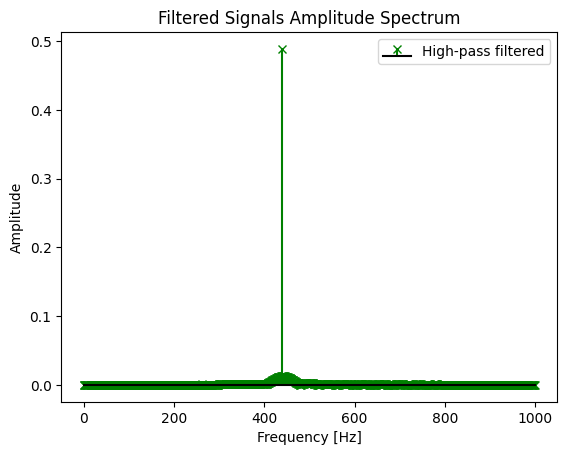
\includegraphics[width=0.6\textwidth]{fig_28.png}
      \caption{作成したハイパスフィルタ $h_hpf[n]$ を適用し得た畳み込み和の振幅スペクト}
      \label{fig:fig7}
    \end{figure}

    \begin{figure}[!h]
      \centering
      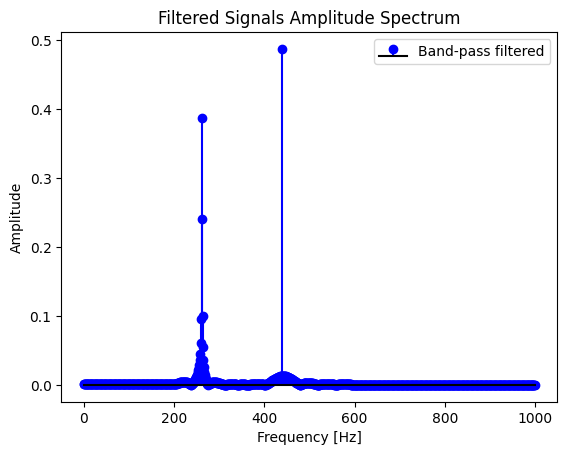
\includegraphics[width=0.6\textwidth]{fig_27.png}
      \caption{作成したバンドパスフィルタ $h_bpf[n]$ を適用し得た畳み込み和の振幅スペクトル $H_bpf[k]$}
      \label{fig:fig8}
    \end{figure}
  
    \subsection*{考察}
    
      図 \ref{fig:fig7} を,課題2-2 の $|X_{add}[n]|$ の図 \ref{fig:fig2} と比較すると, $F = 360 [\mathrm{Hz}]$ 以下のド ($ = 261.626 [\mathrm{Hz}]$) に対応する位相スペクトルのピークはカットされ,ラ ($ = 440 [\mathrm{Hz}]$) に対応する位相スペクトルのピークは残されていることが確認できる.
  
      このことから,ハイパスフィルタが正しく設計され,適用されていることがわかる.

      また,図 \ref{fig:fig8} を,課題2-2 の $|X_{add}[n]|$ の図 \ref{fig:fig2} と比較すると, ド ($ = 261.626 [\mathrm{Hz}]$) および ラ ($ = 440 [\mathrm{Hz}]$) に対応する位相スペクトルのピークはいずれも残されていることが確認できる.

      これは,作成したバンドパスフィルタと矛盾しないといえる.

  \newpage

  \section*{課題3-1: ナイキスト周波数}

  $4 [\mathrm{Hz}]$ の正弦波を 1 秒あたり 32 点,6 点のそれぞれで,サンプリング周波数を変化させてサンプリングした.

  図 \ref{fig:fig9} は,それぞれのサンプリング周波数における離散時間信号 $x_{32}[n], x_{6}[n]$ とそれらの離散フーリエ変換の振幅スペクトル $X_{32}[k], X_{6}[k]$ をプロットしたものである.

  \begin{figure}[!h]
    \centering
    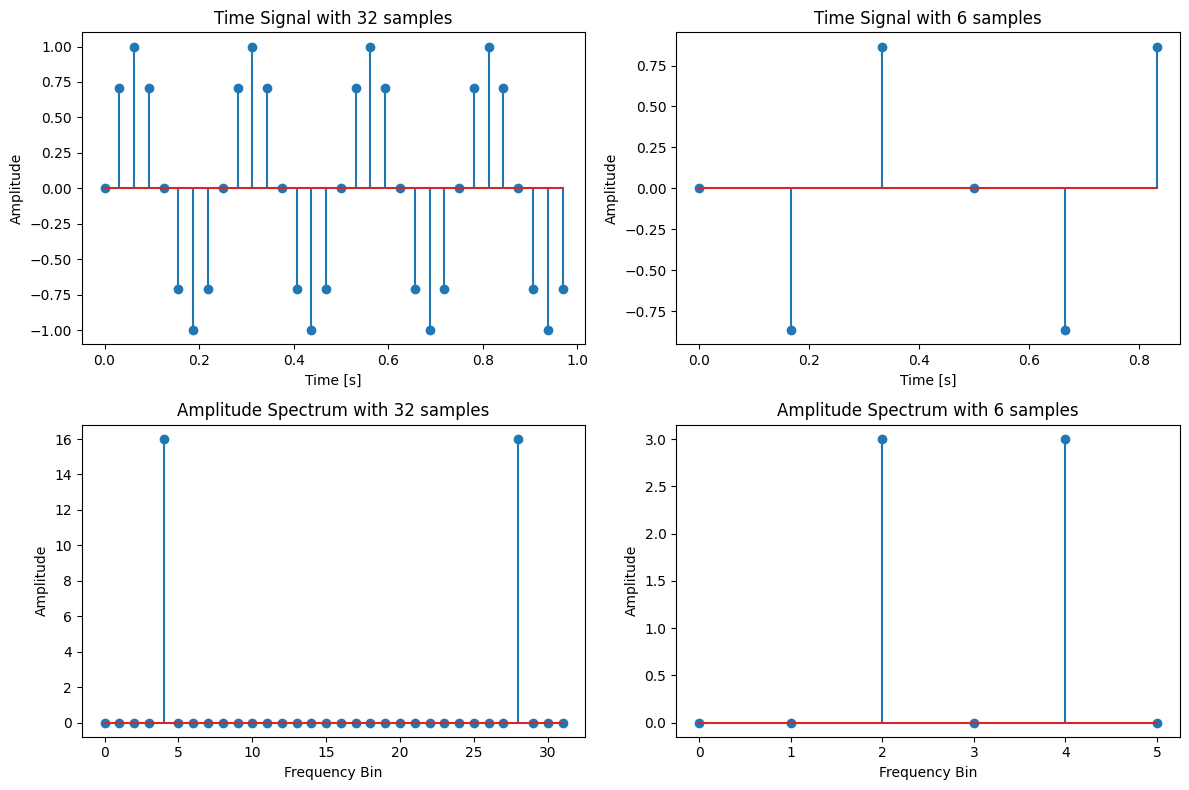
\includegraphics[width=1\textwidth]{fig_3_1.png}
    \caption{$4 [\mathrm{Hz}]$ の正弦波を 1 秒あたり 32 点,6 点でサンプリングしたときの離散時間信号 $x[n]$ とその離散フーリエスペクトルの振幅スペクトル $|X[k]|$}
    \label{fig:fig9}
  \end{figure}

  \subsection*{考察}

    $F_s$ をサンプリング周波数,$F_N$ をナイキスト周波数,$F_m$ を離散時間信号 $x[n]$ から復元可能な最小のサンプリング周波数と定義する.
    
    まず,ナイキスト周波数の定義は,以下の通りである.

    \begin{equation}
      F_N = \frac{F_s}{2}
    \end{equation}

    ここで,ナイキストシャノンのサンプリング定理によれば,離散時間信号 $x[n]$ の最高周波数が,ナイキスト周波数 $F_N$ を超えないとき,元の信号を復元することができる.

    ここでは,離散時間信号 $x_{32}[n]$ および $x_{6}[n]$ の最高周波数は,題意より,$4 [\mathrm{Hz}]$ である.

    したがって,復元可能な最小のサンプリング周波数は, $F_m = 8 [\mathrm{Hz}]$ である.

    よって,$F_s = 32 [\mathrm{Hz}]$ は,$F_m = 8 [\mathrm{Hz}]$ を超えているため,元の信号を復元することができる.
    
    一方,$F_s = 16 [\mathrm{Hz}]$ は,$F_m = 8 [\mathrm{Hz}]$ を下回っているため,元の信号を復元することができない.

    \newpage

    \section*{課題3-2: DFT という変換対}

    次に,課題3-1 において求めた,離散時間フーリエスペクトル $X_{32}[k], X_{6}[k]$ を逆フーリエ変換して,元の信号の復元を試みる.

    図 \ref{fig:fig10} は,離散時間フーリエスペクトル $X_{32}[k], X_{6}[k]$ それぞれの逆フーリエ変換によって得られた時間信号である.
  
    \begin{figure}[!h]
      \centering
      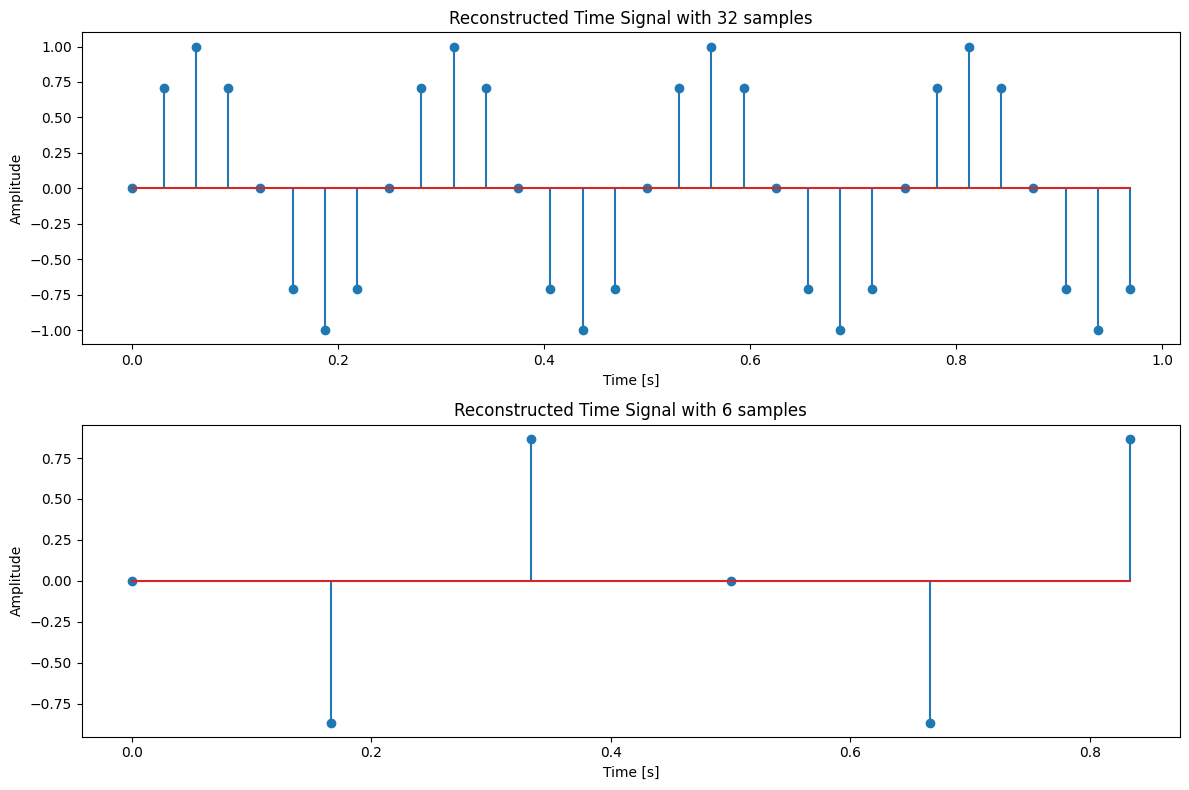
\includegraphics[width=1\textwidth]{fig_3_2.png}
      \caption{離散時間フーリエスペクトル $X_{32}[k], X_{6}[k]$ それぞれの逆フーリエ変換によって得られた時間信号}
      \label{fig:fig10}
    \end{figure}
  
    \subsection*{考察}
  
      図 \ref{fig:fig10} より,$F_s = 32 [\mathrm{Hz}]$ のとき,元の信号を復元することができている.
  
      一方,$F_s = 16 [\mathrm{Hz}]$ のとき,元の信号を復元することができていない.
  
      これは,課題3-1 で述べた通りであり,ナイキストシャノンのサンプリング定理によって,元の信号を復元するためには,サンプリング周波数がナイキスト周波数を超えている必要があることがわかる.

    \newpage

    \section*{課題3-3: 窓関数}

    次に,窓関数を用いる.

    以下の手順に従い進める.

    \begin{enumerate}
      \item $4 [\mathrm{Hz}]$ の正弦波と $6 [\mathrm{Hz}]$ の正弦波を合成した信号を生成した.
      \item 生成した信号 $x_{add}[n]$ を,$n = 7, \dots, 29$ の 23 点でサンプリングした $x_{cut}[n]$ について,その DFT の振幅スペクトルを求めた.
      \item $x_{cut}[n]$ に,ハニング窓 $w[n]$ を適用した $x_w[n]$ について,その DFT の振幅スペクトルを求めた.
    \end{enumerate}

    図 \ref{fig:fig11} は,$x_{add}[n], x_{cut}[n], x_w[n]$ それぞれの離散時間信号および, DFT の振幅スペクトルをプロットしたものである.
  
    \begin{figure}[!h]
      \centering
      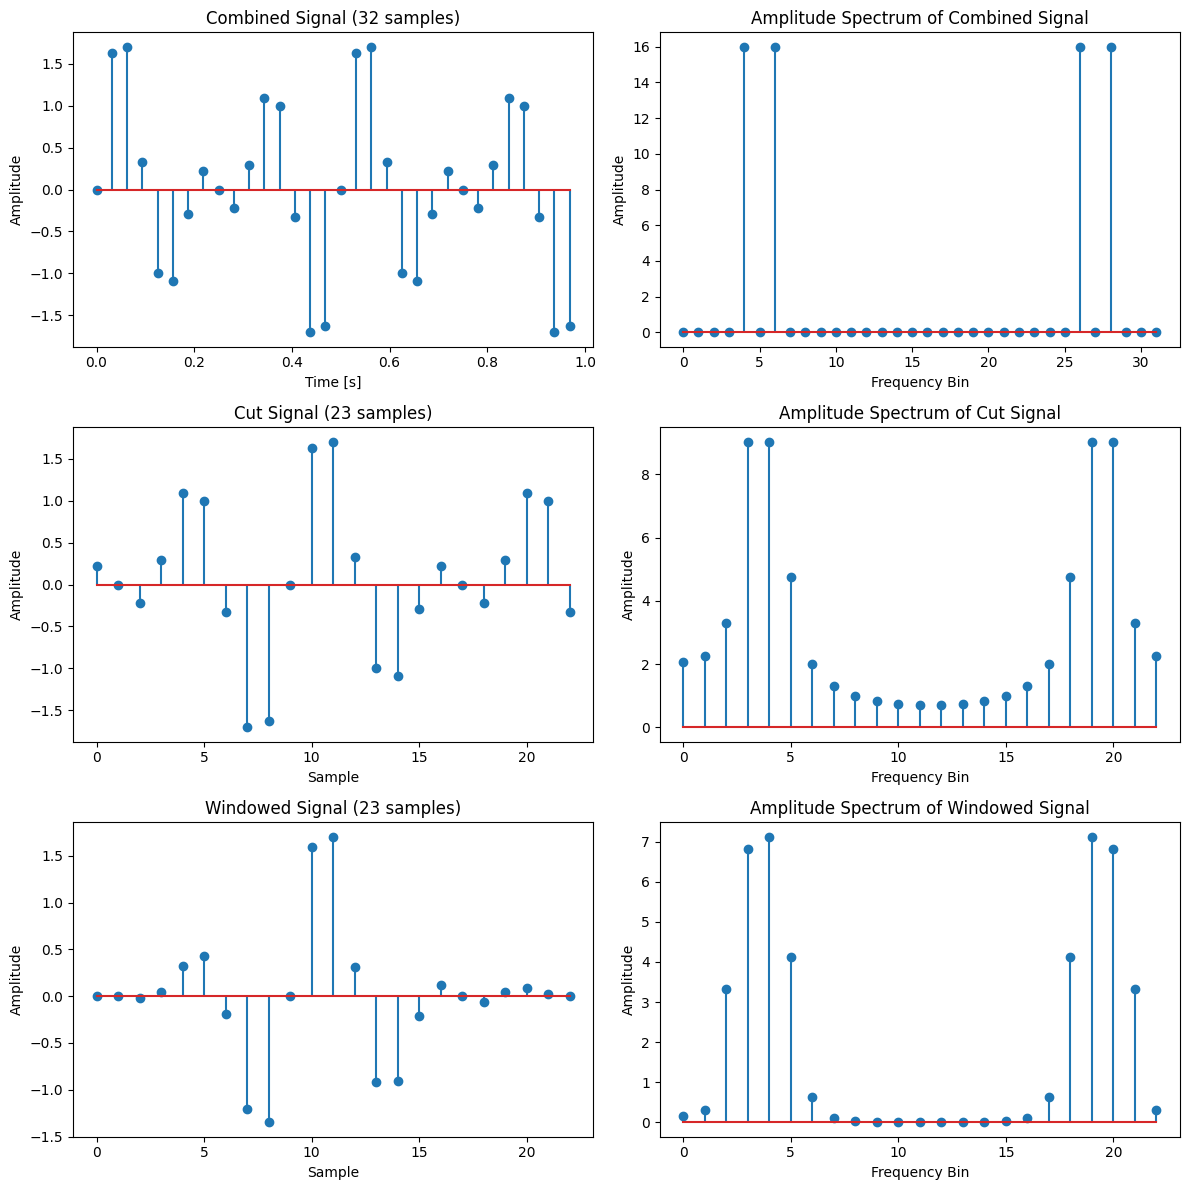
\includegraphics[width=1\textwidth]{fig_3_3.png}
      \caption{$x_{add}[n], x_{cut}[n], x_w[n]$ それぞれの離散時間信号および, DFT の振幅スペクトル}
      \label{fig:fig11}
    \end{figure}
  
    \subsection*{考察}
  
      図 \ref{fig:fig11} より,$x_{add}[n]$ には,周期性が存在するため,DFT の振幅スペクトルには,$F = 4 [\mathrm{Hz}]$ および $F = 6 [\mathrm{Hz}]$ のピークが生じている.

      一方,$x_{cut}[n]$ には,周期性がないため,DFT の振幅スペクトルには,ピークが多数生じている.

      窓関数を用いることで,$x_w[n]$ では,始端と終端の調整が行われたことで,DFT の振幅スペクトルにおいて,ピークの有無がはっきりし,完璧ではないものの, $x_{add}[n]$ の DFT の振幅スペクトルに近くなっている.

  \newpage

  \section*{おわりに}

    本実験では,離散フーリエ変換を用いて,周期信号および非周期信号の周波数成分を解析することを通して,アナログとデジタル間の変換といった信号処理の基礎を学ぶことができた.

    アナログな信号を,デジタルな信号に,情報欠損なしで変換することができることにおける,フーリエ変換の有用性が印象的だった.

    また,このように情報が失われずに,デジタルな信号に変換するためには,ナイキスト周波数を超えるサンプリング周波数が必要であることがわかった.

  \newpage
  
  \section*{参考文献}

    \begin{itemize}
        \item Numpy and Scipy Documentation - https://docs.scipy.org/doc/ (accessed 2024-06-19)
    \end{itemize}

\end{document}